%!TEX root = ../these.tex

\chapter{
  Задача оптимизации маршрута
  режущего инструмента
  для машин термической резки с ЧПУ
}
\label{ch:review}

\lipsum

\section{Oops}

\begin{table}[h!]
  \centering
  \caption{Сравнение качества решений задач CCP и GTSP}
  \label{tab:ccp-vs-gtsp}
  \def\arraystretch{1.2}
  \begin{tabular}{l|*{3}{r}}
      Задание & № 229 & № 464 & № 3211 \\
      \hline
      Кол-во деталей & 11 & 14 & 17\\
      Кол-во контуров & 12 & 21 & 22 \\
      Общий периметр, м & 24.609 & 21.717 & 25.051 \\
      Кол-во точек GTSP & 491 & 429 & 493 \\
      $\mathcal L_{GTSP}$, м & 7.729 & 4.743 & 4.557 \\
      $\mathcal L_{CCP}$, м & 7.727 & 4.706 & 4.536 \\
      \hline
  \end{tabular}
\end{table}

\begin{figure}
  \centering
  \includegraphics[width=0.95\textwidth]{classes.pdf}
  \caption{Классификация задач резки}
  \label{fig:cut-classes}
\end{figure}
